\documentclass[../main.tex]{subfiles}

\begin{document} %%%%%%%%%%%%%%%%%%%%%%%%%%%%%%%%%%%%%%%%%%%%%%%%%%%%%%%%%%%%
\section{Java} 
    % Cargamos una imagen
    \begin{figure}[h]
        \centering
        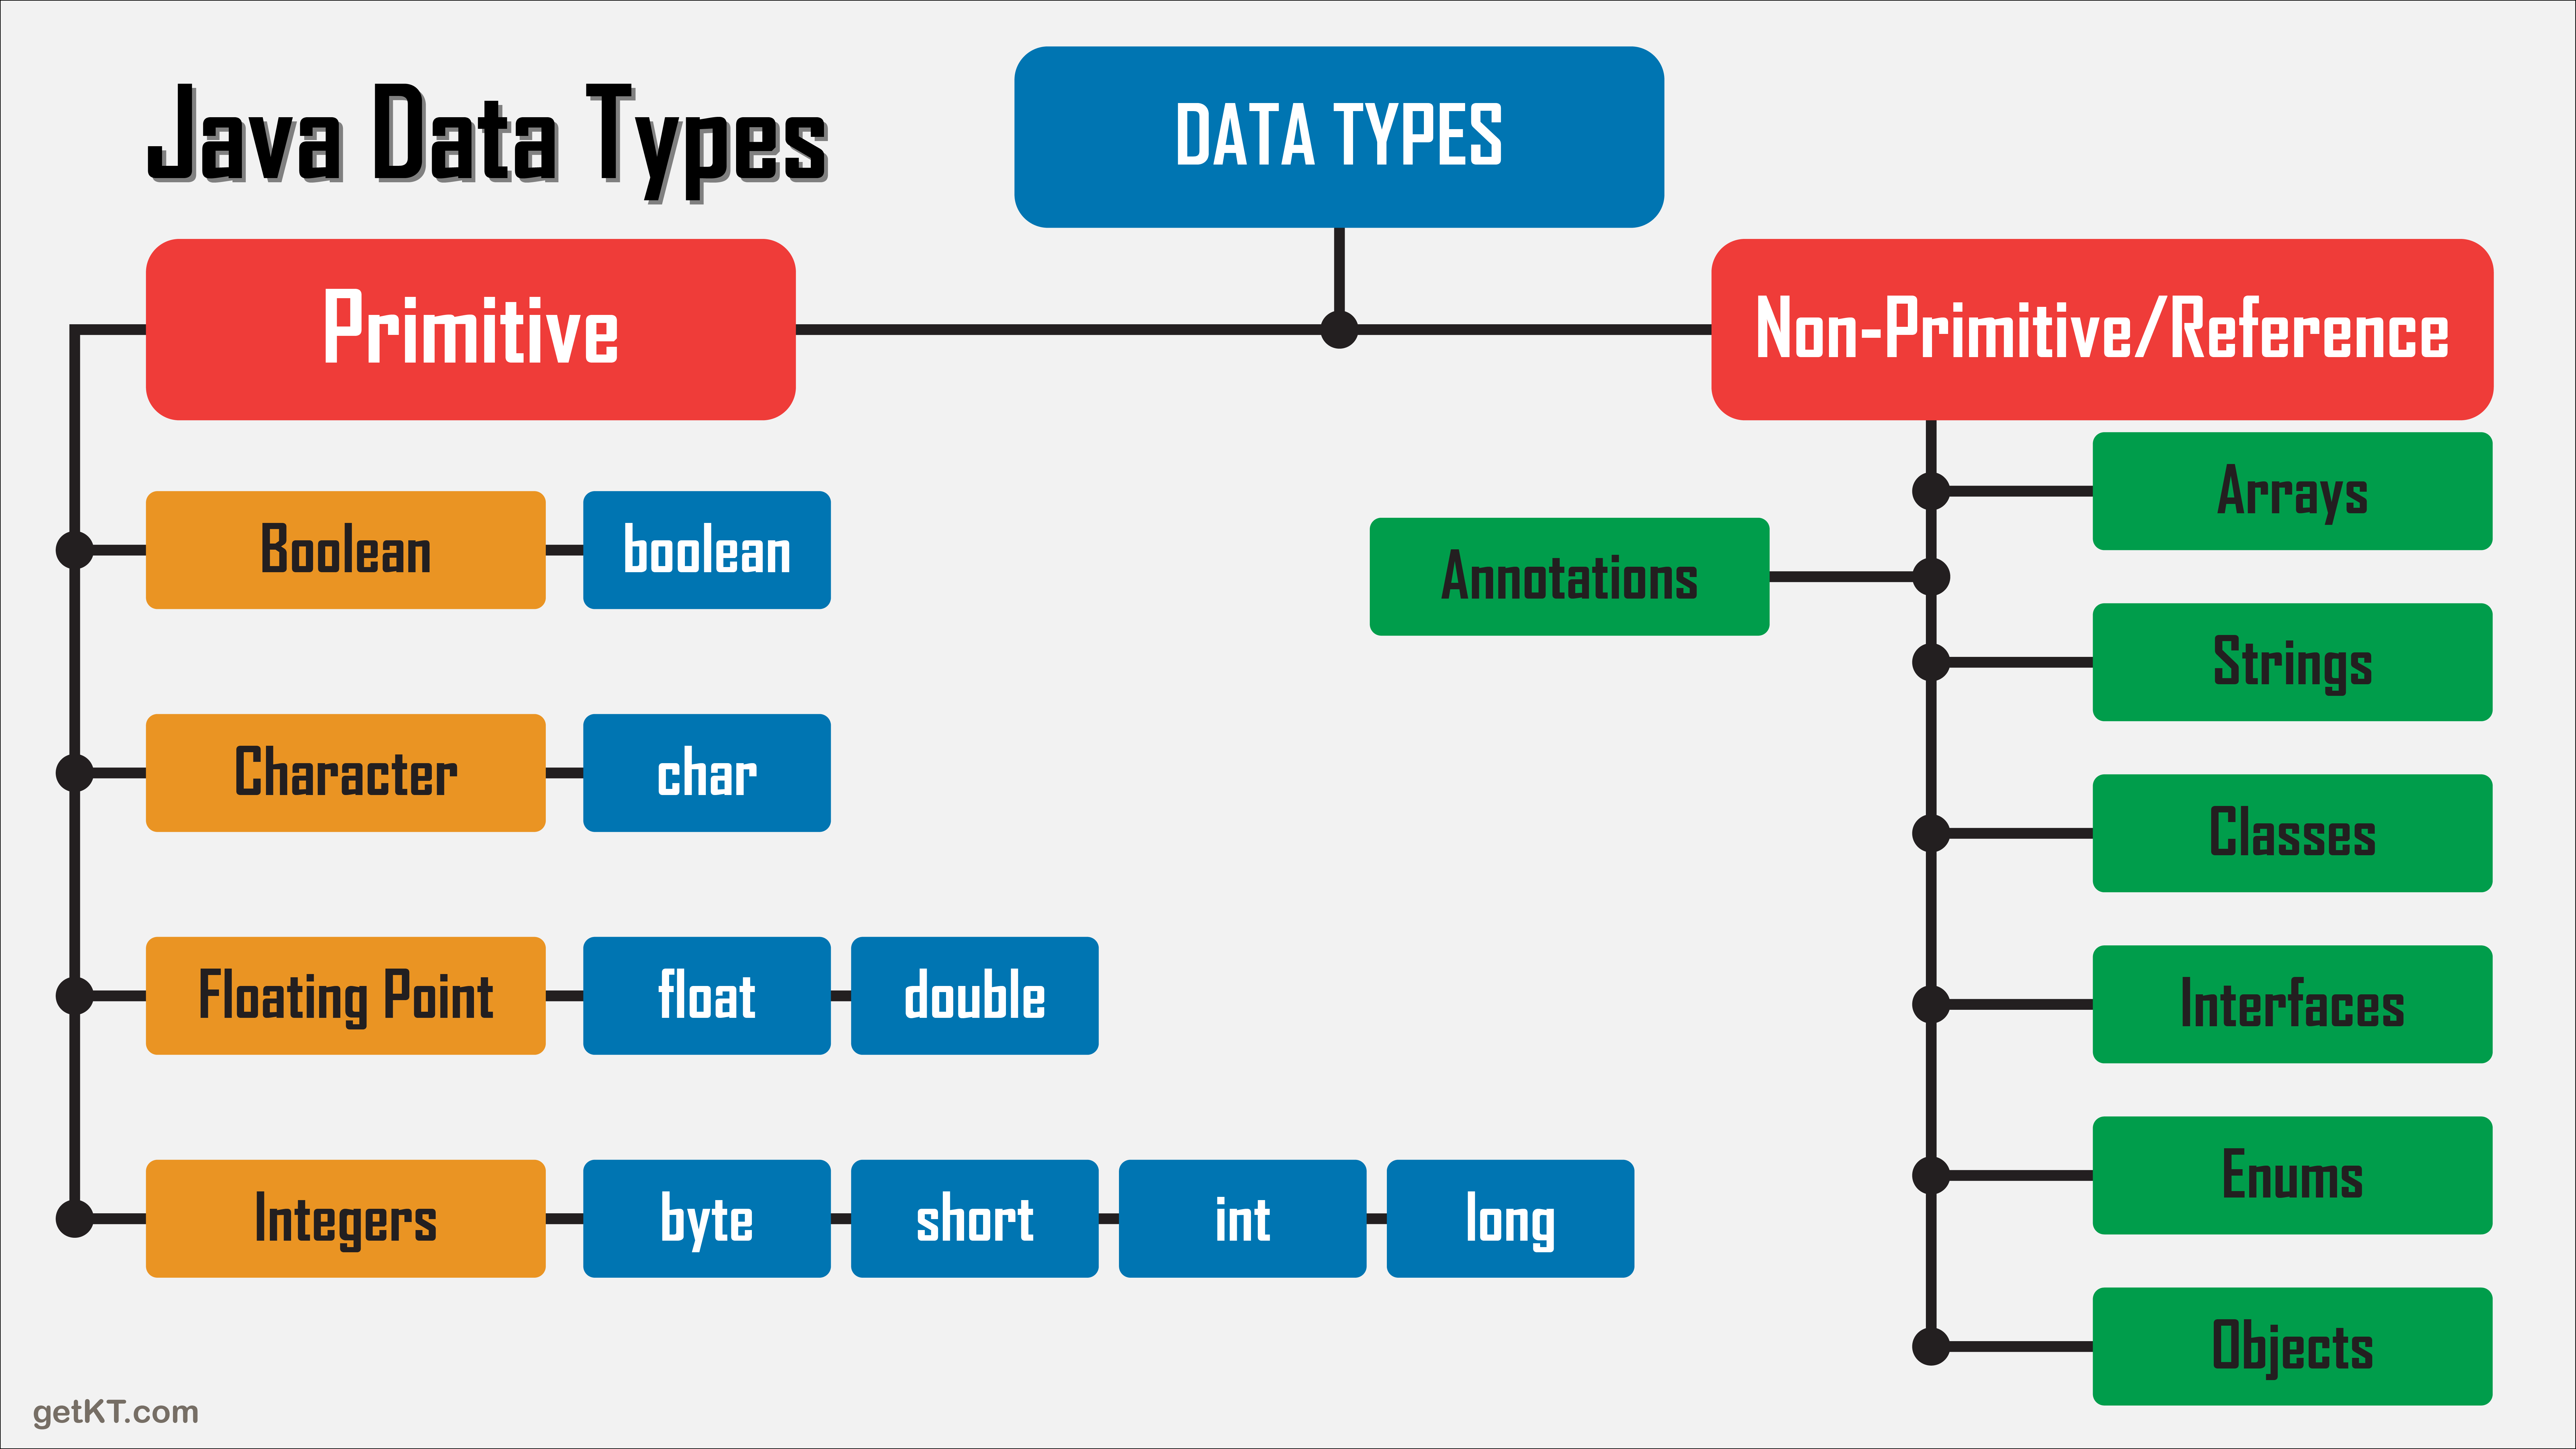
\includegraphics[width=0.8\textwidth]{../images/tipos_datos.png}
        \caption{Tipos de datos en Java \cite{tipos_de_datos_primitivos}}
        \label{fig:java}
    \end{figure}

    \subsection{Tipos de clases en JAVA}
        \begin{itemize}
            \item \textbf{Clases}: Son las clases comunes y corrientes, que se pueden instanciar.
            \item \textbf{Clases Abstractas}: Son clases que no se pueden instanciar, pero que sirven para heredar.
            \item \textbf{Interfaces}: Son clases que no se pueden instanciar, pero que sirven para heredar.
            \item \textbf{Clases Anónimas}: Son clases que no tienen nombre, y se usan para sobreescribir métodos.
            \item \textbf{Clases finales}: Son clases que no se pueden heredar.
        \end{itemize}

    \subsection{Relaciones entre clases}
        Relaciones en UML: \cite{uml_relacion_clases}
        \begin{enumerate}
            \item \textbf{Asociación:} Indica que una propiedad de una clase contiene una referencia a una instancia (o instancias) de otra clase.
            
            La asociación es la relación más utilizada entre una clase y otra clase, lo que significa que existe una conexión entre un tipo de objeto y otro tipo de objeto. Las combinaciones y agregaciones también pertenecen a las relaciones asociativas , pero las relaciones entre clases de afiliaciones son más débiles que las otras dos.
            
            Hay cuatro tipos de asociaciones : asociaciones bidireccionales , asociaciones unidireccionales , autoasociación y asociaciones de números múltiples.\\
            
            Por ejemplo: coches y conductores, un coche corresponde a un conductor en particular y un conductor puede conducir varios coches.

            \begin{figure}[ht]
                \centering
                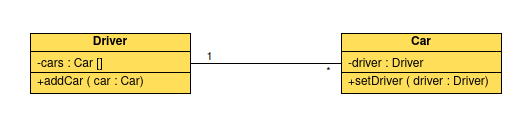
\includegraphics[width=0.7\textwidth]{../images/uml_asociacion.png}
                \caption{Asociación}
                \label{fig:uml_asociacion}
            \end{figure}

                \begin{enumerate}
                    \item \textbf{Agregación:} 
                        La relación entre el todo y la parte, y el todo y la parte se pueden separar.
                        Las relaciones agregadas también representan la relación entre el todo y una parte de la clase, los objetos miembros son parte del objeto general, pero el objeto miembro puede existir independientemente del objeto general.Tiempo de vida \textit{independiente}.\\

                        Por ejemplo, los conductores de autobús y la ropa y los sombreros de trabajo son parte de la relación general, pero se pueden separar. La ropa de trabajo y los sombreros se pueden usar en otros conductores. Los conductores de autobuses también pueden usar otra ropa de trabajo y sombreros.

                        \begin{figure}[ht]
                            \centering
                            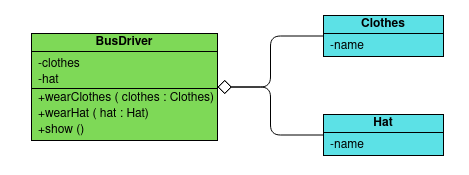
\includegraphics[width=0.7\textwidth]{../images/uml_agregacion.png}
                            \caption{Agregación}
                            \label{fig:uml_agregacion}
                        \end{figure}

                        Otro ejemplo puede ser el de un auto y sus ruedas, el auto depende si o si de tener cuatro ruedas.

                    \item \textbf{Composición:} 
                        La relación entre el todo y la parte, pero el todo y la parte no se pueden separar.
                        
                        La relación de combinación representa la relación entre el todo y la parte de la clase, y el total y la parte tienen una duración constante. Una vez que el objeto general no existe, algunos de los objetos no existirán y todos morirán en la misma vida. Tiempo de vida \textit{dependiente}.\\ 
                        
                        Por ejemplo, una persona está compuesta por una cabeza y un cuerpo. Los dos son inseparables y coexisten. 

                        \begin{figure}[ht]
                            \centering
                            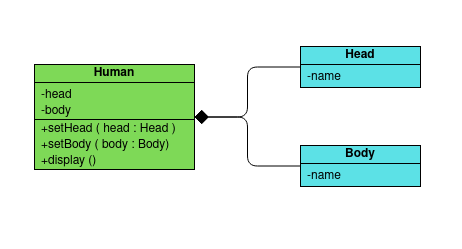
\includegraphics[width=0.7\textwidth]{../images/uml_composicion.png}
                            \caption{Composición}
                            \label{fig:uml_composicion}
                        \end{figure}

                \end{enumerate}
            \item \textbf{Herencia/Generalización:} 
                La herencia también se denomina generalización y se utiliza para describir la relación entre las clases padre e hijo. Una clase principal también se denomina clase base y una subclase también se denomina clase derivada.

                En la relación de herencia, la subclase hereda todas las funciones de la clase principal y la clase principal tiene todos los atributos, métodos y subclases. Las subclases contienen información adicional además de la misma información que la clase principal.\\a

                Por ejemplo: autobuses, taxis y automóviles son automóviles, todos tienen nombres y todos pueden estar en la carretera.

            \item \textbf{Dependencia}: 
                Suponga que un cambio en la clase A provoca un cambio en la clase B, luego diga que la clase B depende de la clase A.
                En la mayoría de los casos, las dependencias se reflejan en los métodos de una clase que utilizan el objeto de otra clase como parámetro .
                Una relación de dependencia es una relación de “uso”. Un cambio en una cosa en particular puede afectar a otras cosas que la usan, y usar una dependencia cuando es necesario indicar que una cosa usa otra. \\
                
                Por ejemplo: El auto depende de la gasolina. Si no hay gasolina, el automóvil no podrá conducir.

                \begin{figure}[ht]
                    \centering
                    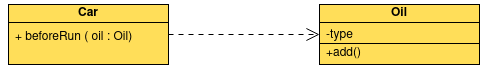
\includegraphics[width=0.7\textwidth]{../images/uml_dependencia.png}
                    \caption{Dependencia}
                    \label{fig:uml_dependencia}
                \end{figure}

            \item \textbf{Realización/Implementación:}
                La implementación (Implementación) se utiliza principalmente para especificar la relación entre las interfaces y las clases de implementación.

                Una interfaz (incluida una clase abstracta ) es una colección de métodos. En una relación de implementación, una clase implementa una interfaz y los métodos de la clase implementan todos los métodos de la declaración de la interfaz.\\
                
                Por ejemplo: los automóviles y los barcos son vehículos, y el vehículo es solo un concepto abstracto de una herramienta móvil, y el barco y el vehículo realizan las funciones móviles específicas.


                \begin{figure}[ht]
                    \centering
                    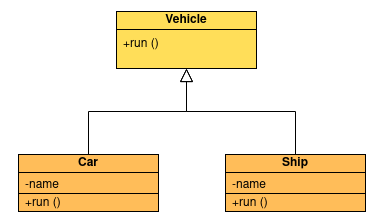
\includegraphics[width=0.5\textwidth]{../images/uml_realizacion.png}
                    \caption{Realización/Implementación}
                    \label{fig:uml_realizacion}
                \end{figure}
        \end{enumerate}

        \begin{figure}[ht]
            \centering
            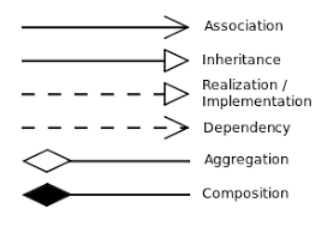
\includegraphics[width=0.5\textwidth]{../images/uml_relaciones.png}
            \caption{UML Relaciones entre clases}
            \label{fig:uml_relaciones}
        \end{figure}


    \subsection{Interface}
        Interfaces: \cite{interfaces}.
        \begin{itemize}
            \item Son una \textbf{colección de métodos abstractos} con propiedades (atributos) \textbf{constantes}.
            \item Una interfaz \textbf{solamente puede extender o implemtar otras interfaces} (la cabtidad que quiera).
            \item Da a conocer qué se debe hacer (métodos) \textbf{pero sin mostrar su implemtación} (solo puede tener métodos abstractos).
            \item Solo puede tener \textbf{métodos} con \textbf{métodos públicos} (no pueden ser protected o private).
            \item Solo puede tener "variables" public static final (o sea constantes).
            \item La palabra tener \textbf{abstract} en la definición de métodos \underline{no es obligatoria}.
            \item Generalmente las interfaces indican el \textbf{PUEDE HACER} de un objeto.
        \end{itemize}






\end{document}  %%%%%%%%%%%%%%%%%%%%%%%%%%%%%%%%%%%%%%%%%%%%%%%%%%%%%%%%%%%%%
